\documentclass{article}
\usepackage[utf8]{inputenc}
\usepackage{graphicx}

\title{Lab 1 Redes}
\author{Vicente Lopez\\Esteban León\\Nicolas Ramírez\\Profesor: Jose Alejandro Perez\\Ayudante: Alexis Inzunza}
\date{Abril 2017}

\usepackage{natbib}
\usepackage{graphicx}

\begin{document}
\begin{figure}[h]

\includegraphics[width=0.45\textwidth]{logo_udp.png}
\maketitle
\end{figure}

\section{Indice}
2 Actividades del laboratiorio--------------------------1\\
2.1 Identificacion de elementos de red----------------1\\
2.1.1 equipo conectado a la red------------------------1\\
2.1.2 switch de la topologia-----------------------------2\\
2.1.3 Hadware de red-------------------------------------2\\
2.1.4 Cableado utilizado---------------------------------3\\
2.1.5 patch panel------------------------------------------3\\
2.2 Informacion de los dispositivos--------------------3\\
2.3 Diagrama de red--------------------------------------4\\
3 Conclusion------------------------------------------------4\\
\section{Actividad de laboratorio}
\subsection{Identificacion de elementos de red}
\subsubsection{Equipo conectado a la red}
En el laboratorio de informatica existe 18 equipos conectados a la red, de modo que cada uno de estas maquinas estan conectadas a una switch atraves de una canaleta \\
\subsubsection{Switch de la toplogia}
El switch esta ubicada a una equina de la sala, en una caja llamada Rack como se logra apreciar en la siguiente imagen enmarcado en un cuadro rojo\\
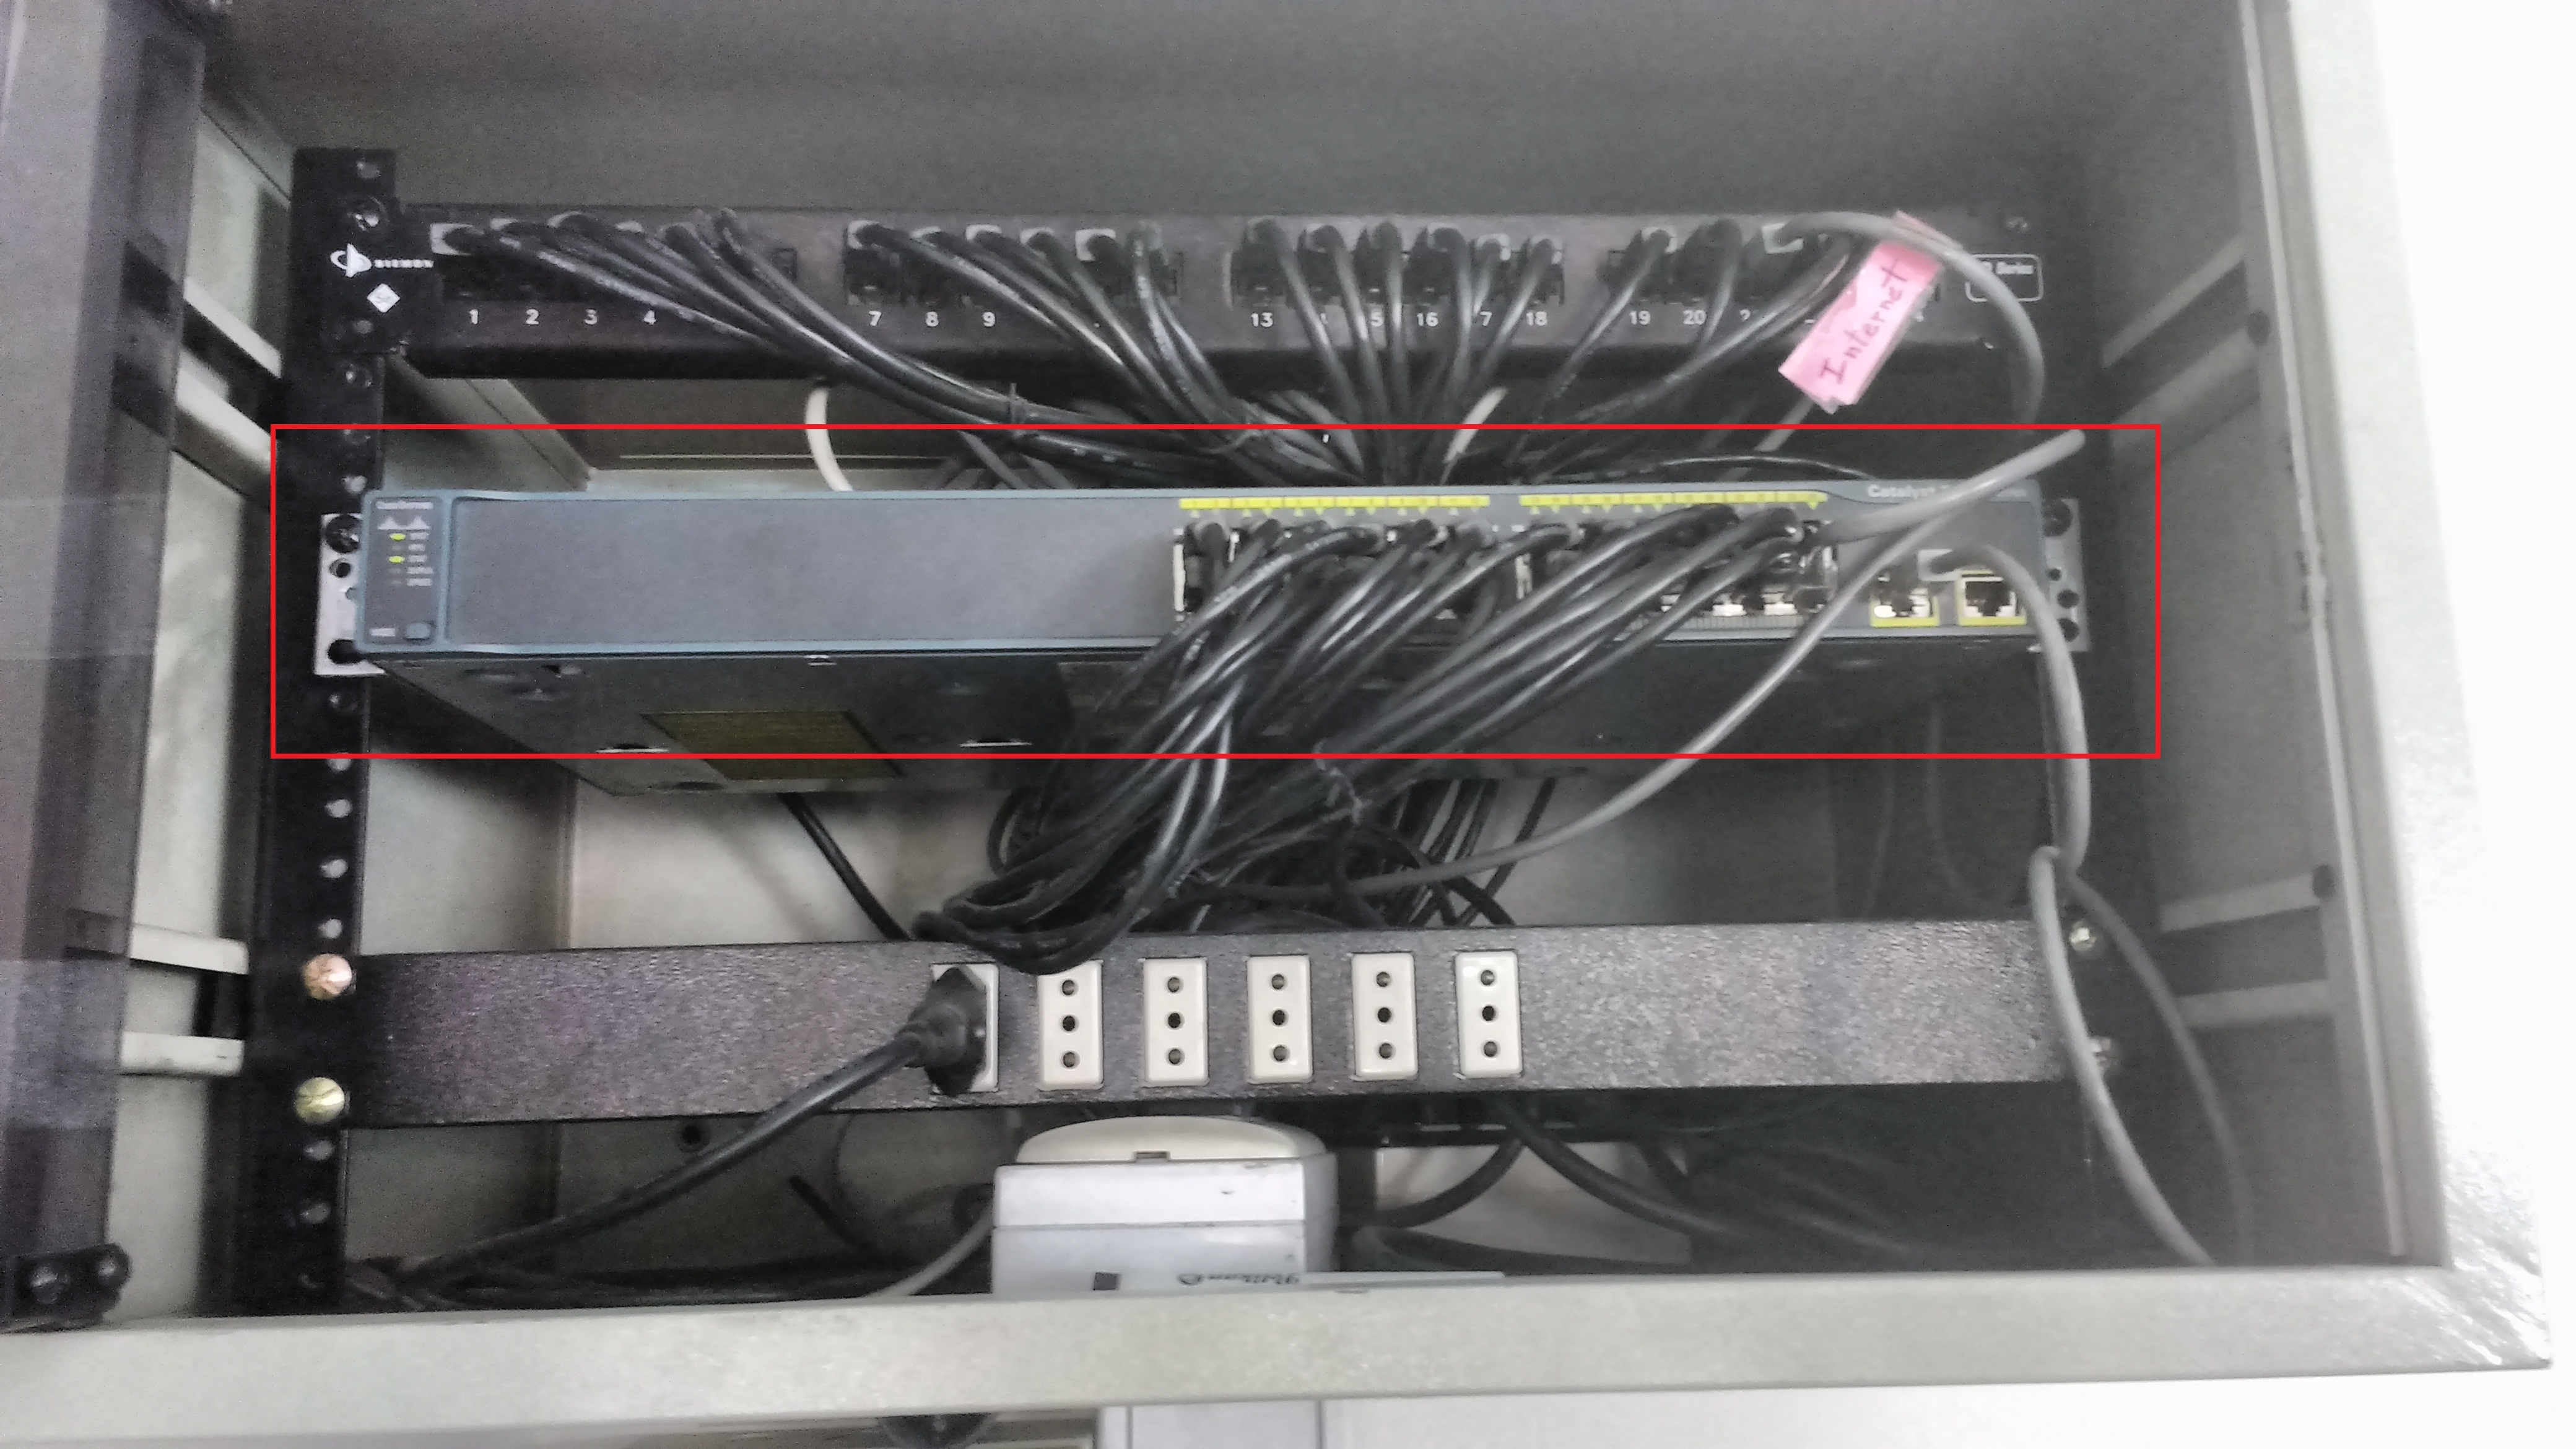
\includegraphics[width=11cm, height=6cm]{switch.jpg}
\subsubsection{Hadware de red}
El hadware de red es identificado mediante un marco de color rojo en la siguiente imagen\\ \\ 
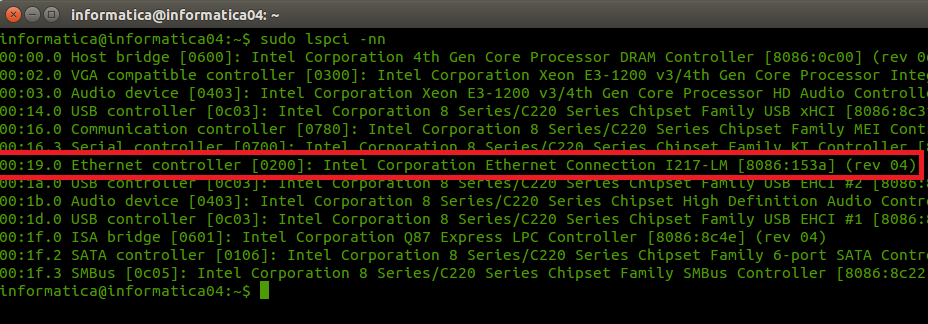
\includegraphics[width=16cm, height=7cm]{Tar_de_Red.png} \\ \\ \\
\subsubsection{Cableado utilizado}
Los cables ultilizados son UTP categoria 5E\\ \\
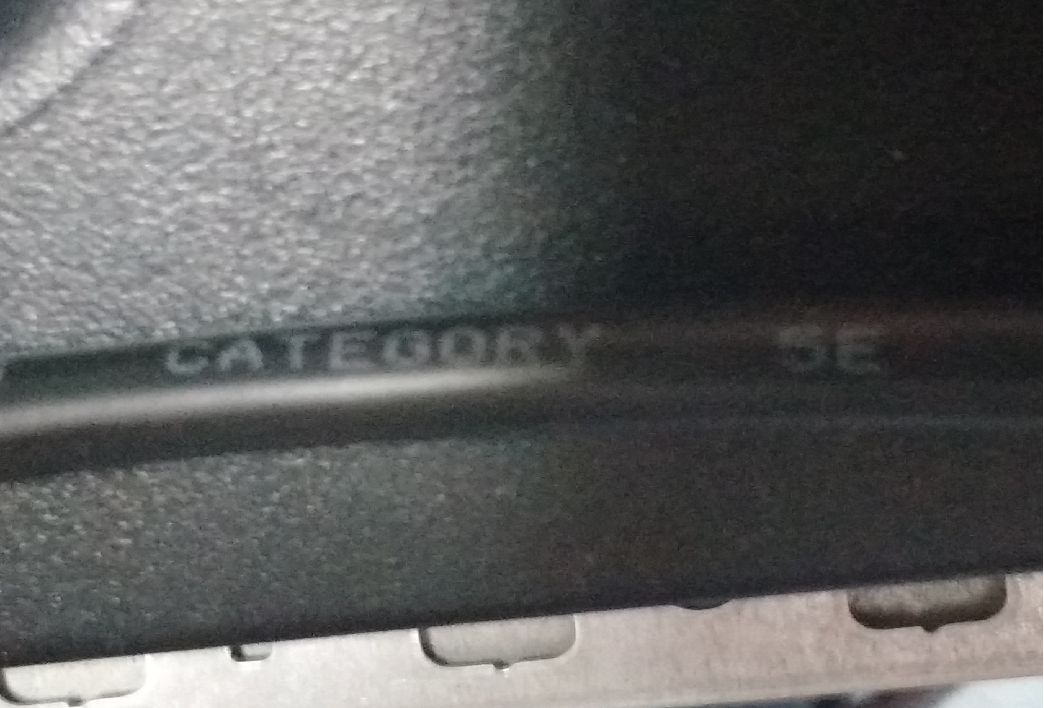
\includegraphics[width=5cm, height=5cm]{Cat_5E.png}
\subsubsection{Patch panel}
Al igual que la Switch, el patch panel esta ubicado en el Rack como se ve en la siguiente imagen enmarcado en un cuadro rojo\\ \\ 
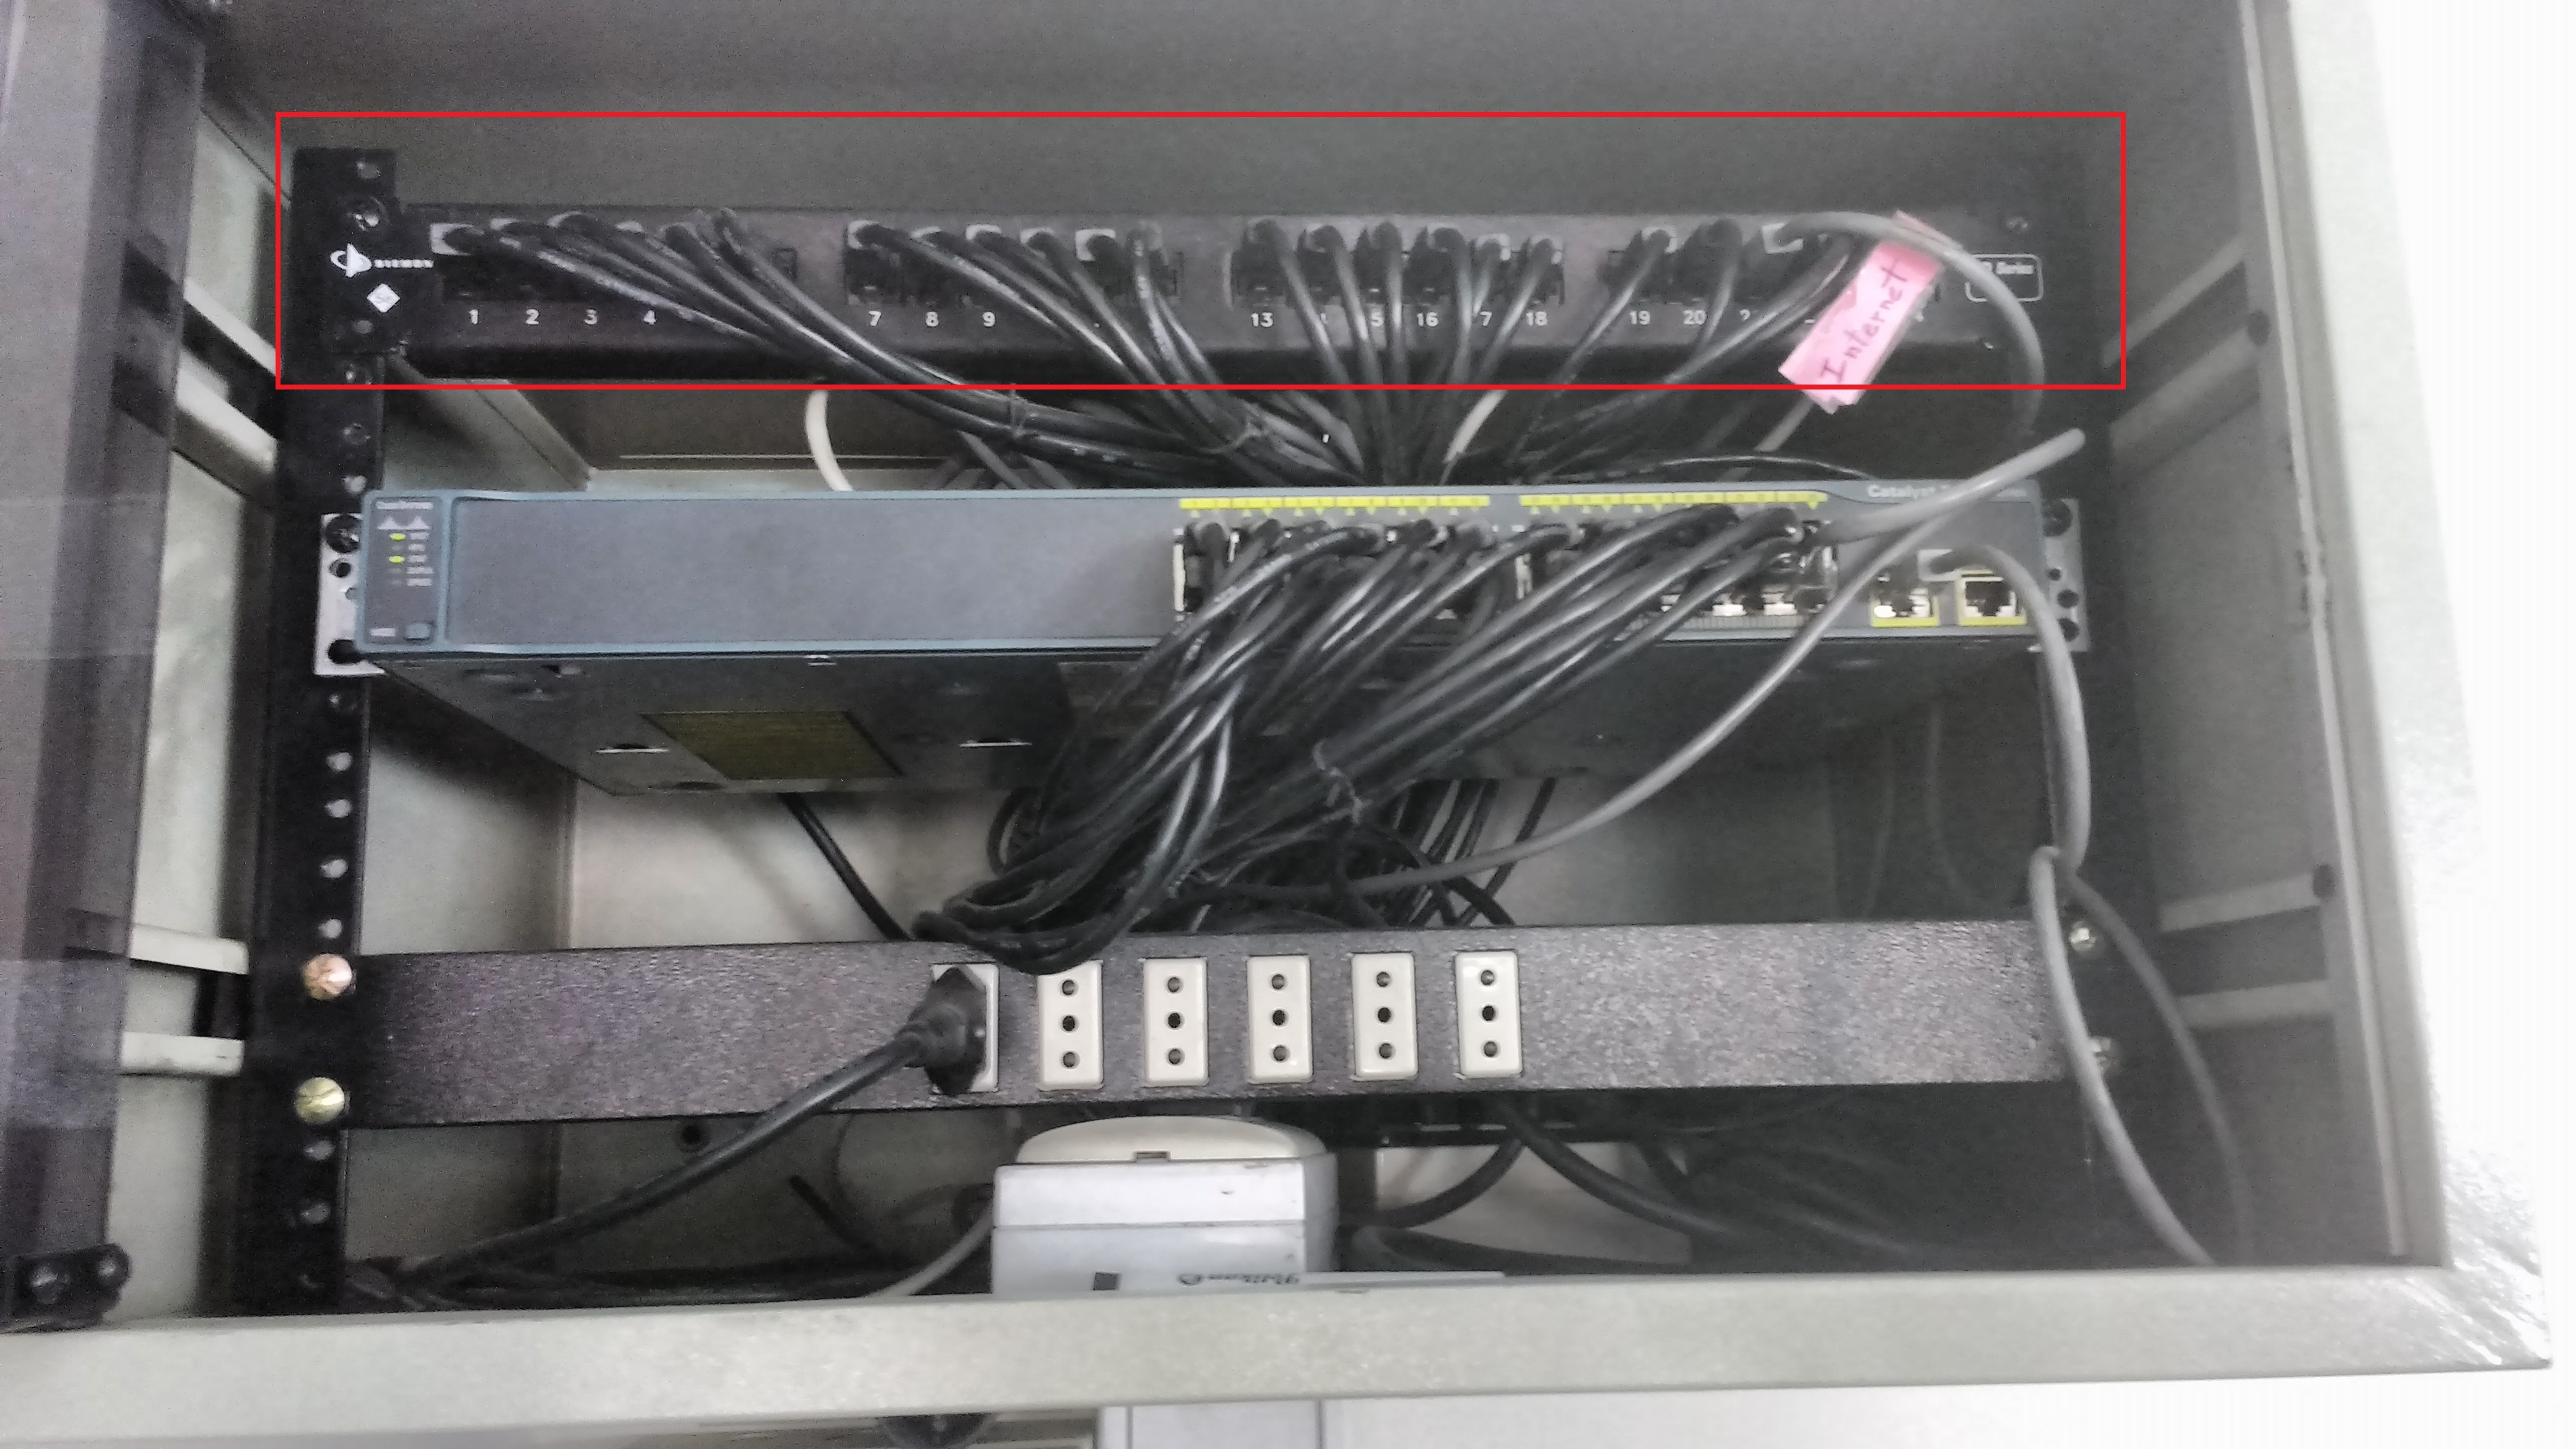
\includegraphics[width=11cm, height=6cm]{pp.jpg}
\subsection{informacion de los dispositivos}
Luego de abrir la consola en Linux y escribir "ifconfig", se mostro la configuracion de la red, en donde la imagen presentada a continuacion, lo que esta subrayado en rojo es la MAC y en azul el IPv4\\
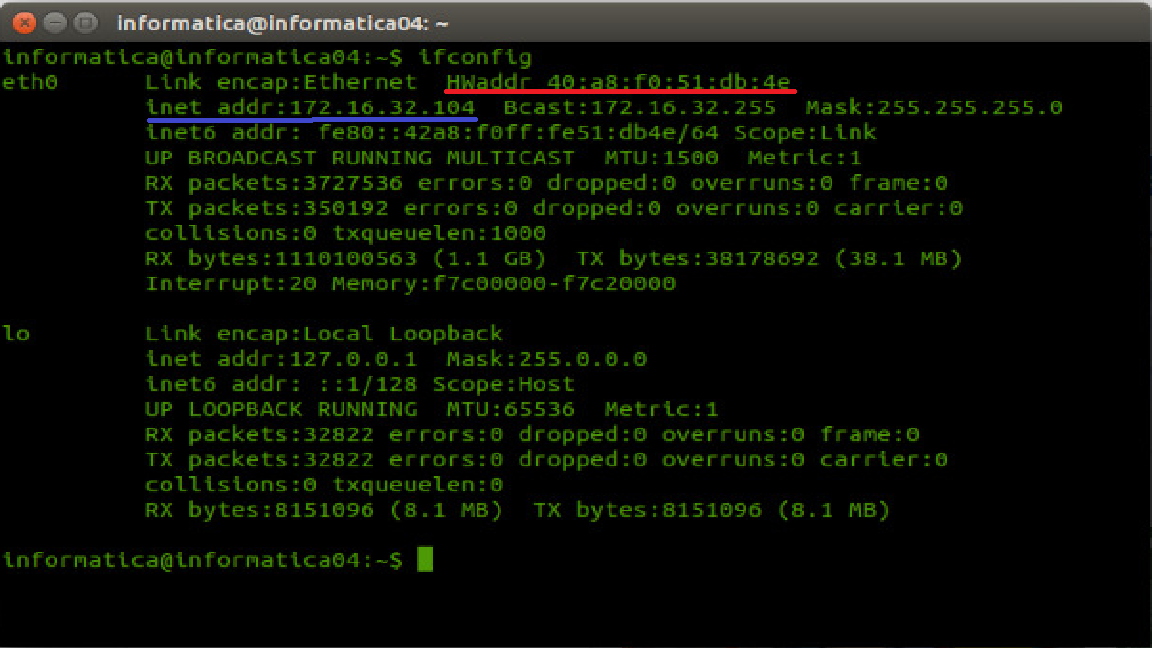
\includegraphics[width=11cm, height=6cm]{Mac_IP.png}

\subsection{Diagrama de red}
El diagrama de red presente en la sala es de topologia de tipo estrella, tanto fisica y loqicamente \\ \\
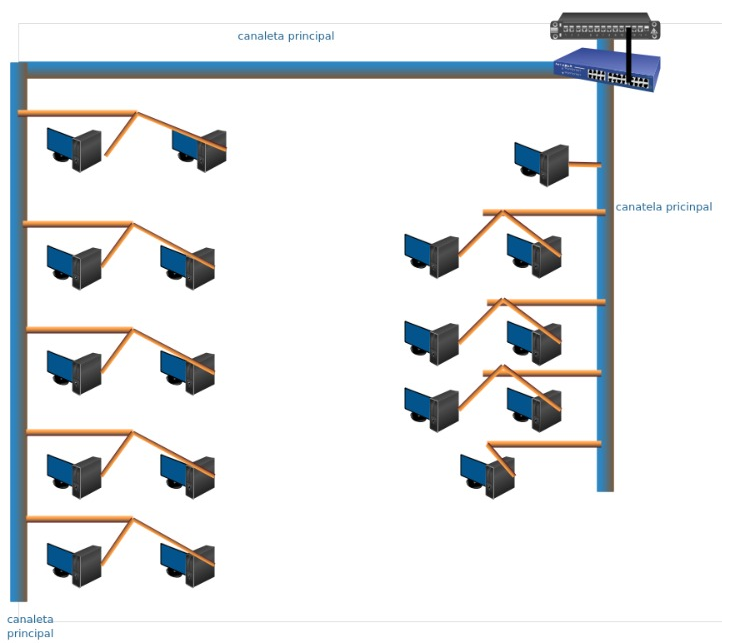
\includegraphics[width=8cm, height=7cm]{Top_fi.png}
\section{Conclusion}
Luego de realizar las actividades del laboratorio, logramos identificar los elementos de red,conseguir la direcion IP y MAc de un equipo y finalmente en el diagrama de red se logra concluir que la sala posee una topologia tanto fisica como logica de tipo estrella


\end{document}